\maketitle
\section*{The Universe}
In the beginning the Universe was created. This has made a lot of people very angry and been widely regarded as a bad move.
I know what I did to make so many people so angry, but it really just sounds like their problem.

In figure \ref{fig:universe} you can see a picture of a galaxy.

\begin{figure}[h]
  \center
  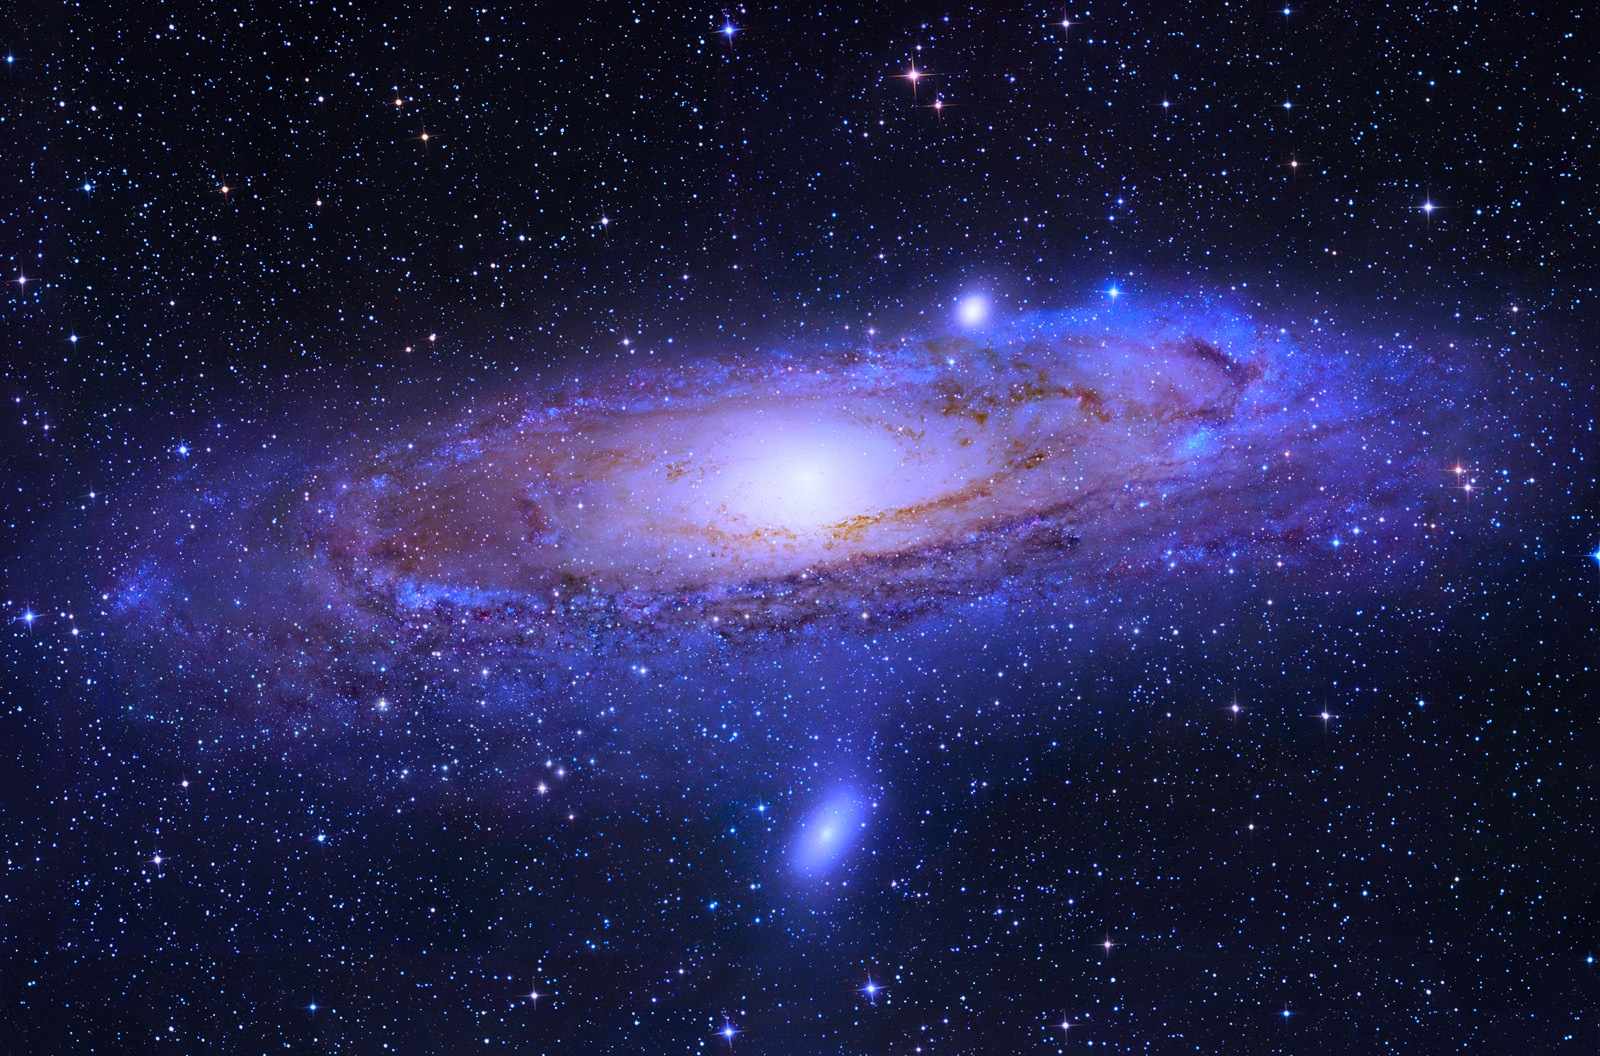
\includegraphics[width=0.6\textwidth]{galaxy.jpg}
  \caption{A picture of a galaxy}
  \label{fig:universe}
\end{figure}

A galaxy is really big. You're just a tiny spec of dust in comparison. Now, there are a lot of galaxies in the universe.
So many indeed, that there are galaxy clusters, where multiple galaxies are grouped together based on the distance between them.
But that's not enough yet. There are also clusters of clusters. And then there's groups of clusters.

The universe is really big. We don't even really know how big. Why? We can't even see it's borders, because light from there hasn't reached us yet.

In a believed stroke of genius, some may say that there's still something more massive, your mom. However, since we're here to proof that you're insignificant,
your mom can't be this massive, or it would be something you'd be significant for.

\pagebreak

\section{The Beginning}

Now let's talk about how everything came to be. Since, you know, I'm God, I have utmost authority when speaking about how things came to be.

Now, in another believed stroke of genius, some may say that everything came to be, because I fucked your mom. However, I'm God, so I have higher standards.

What actually happened, is that I just felt like torturing some innocent souls of the aether for existing, so I just made an endless place of torment to place them into.
This has backfired immensly though, because somehow, somewhy, some people believe that there's a way to salvation and that I love them and so on. I don't realy know how the fuck
you'd think that, but you do you. Now I could end this paper here and have you conclude on your own that you're insignificant, because I obviously created you to torture you, but
I feel like shitting on you some more, so this is only \emph{the Beginning}.

\begin{center}
  Have fun!
\end{center}
\section{Your Beginning}

It doesn't matter.